\documentclass[openany,notitlepage]{book}

\usepackage[margin=2cm]{geometry}
\usepackage{xurl}
\usepackage{enumitem}
\usepackage{graphicx}
\setlist{itemsep=0.5pt}
\usepackage{imakeidx}
\usepackage{xcolor}
\usepackage[hang]{footmisc}
\usepackage{hyperref}
\hypersetup{
	colorlinks = true,
	linkcolor = blue,
	urlcolor = blue
}

\makeatletter
\newcommand*{\toccontents}{\@starttoc{toc}}
\makeatother

\makeindex[intoc]

\usepackage{tikz}
\usetikzlibrary{shapes.geometric, arrows, positioning, calc}
\tikzstyle{startstop} = [rectangle, rounded corners, minimum width=2cm, minimum height=0.5cm,text centered, draw=black]
\tikzstyle{io} = [trapezium, trapezium left angle=70, trapezium right angle=110, minimum width=3cm, minimum height=0.5cm, text centered, draw=black]
\tikzstyle{process} = [rectangle, minimum width=3cm, minimum height=0.5cm, text centered, draw=black]
\tikzstyle{decision} = [diamond, minimum width=3cm, minimum height=1cm, text centered, draw=black]
\tikzstyle{arrow} = [thick,->,>=stealth]



\begin{document}
	\title{Notes on ``Arranger'' 1.1.2}
	\author{Xinyuan Zhou}
	\maketitle
	
	\noindent{\large\textbf{Table of Contents}}

	\toccontents
	
	\chapter{Overview}
	
	\section{What this Project Does}
	So\ldots{} my teacher's rules for rooming on a very specific field trip that I am not going to disclose is as follows:
	\begin{itemize}
		\item No boys sleep with girls. (This is trivial to come up with, I guess).
		\item Most rooms by grade level, but people can \emph{request} to sleep with people from other grade levels, and a very limited number of people can do this. We agreed that a numerical priority will be filled in to prioritize those requests, since there is a cap on the number of people that gets to do this.
		\item At most $4$ people per room, wasting minimal rules.
	\end{itemize}
	Therefore, I came up with this approach:
	\begin{itemize}
		\item Let my teacher assign a priority to each cross-grade-level request, sort them from highest to lowest, consider throwing all people involved in the request into the multiple-grade-level pool (one for boys and one for girls), if it causes it to overflow, don't do this request. But we do this in the order of priority.
		\item There's multiple-grade-level boys \& girls and $\{6,7,8\}$th grade boys and girls, and we call each of those a \emph{sector}. A greedy algorithm documented in the \textsc{readme} (and also at section \ref{Algorithm}) gets used to separate those into actual rooms.
		\item To waste minimal rooms, put non-complete rooms into a ``leftovers`` sector and just put them in groups of $4$ (or the room size) artificially. This is only if there's \emph{not} $\geq3$ leftovers in the sector.
		\item Some documents are generated to document those rooms and facilities are provided to change rooms.
	\end{itemize}
	A VBA script is provided to convert to a Word document. Everything is in the form of \verb+txt+ files.
	
	\section{Setup}
	
	Add a new office script, replace the default content with the ones from \verb|Auto-Setup-Script.txt|\index{Auto-Setup-Script.txt} in the root
	directory of the public distribution, and click run. Next, hook up the $4$
	scripts in \verb|app-scripts/| in their respective locations indicated in the workbook set up by the script. To hook up a script, go to the Automate tab, create a new office script, replace its contents with the contents from the appropriate text file, then click on the three dots and choose ``Add in Workbook''.\index{Office Script, hook up}
	
	Setting up the VBA conversion-to-Word thingy: You need to bring up the ``Developer'' tab as described in
	\url{https://support.microsoft.com/en-us/office/show-the-developer-tab-e1192344-5e56-4d45-931b-e5fd9bea2d45}.
	In the Developer tab, click on Visual Basic, on the top-level V.B.\ project on the left, click \texttt{Insert -> Module}. Put the
	code inside from the text file. After that, use the Developer tab to hook up a button (on Windows, use FORMS control).
	Choose "Export" for the macro it triggers.\index{Developer Tab}
	
	Also you must include Microsoft Word object library in your References (see \url{https://learn.microsoft.com/en-us/office/vba/language/how-to/check-or-add-an-object-library-reference}).
	\chapter{The Office Scripts}
	\section{Things to Fill In}
	\subsection{Student Info}\index{Student Info}\label{inf}
	Fill in Columns \verb|A|, \verb|B|, \verb|C|, \verb|D| starting with row \verb|2|. Put the number of students in \verb|F3|,
	multiple-grade-level-quota for boys in \verb|F5|, and the quota for girls in \verb|F7|. All of those are used by the
	program (all $3$ scripts) because they need to lookup info. Fill in Boy or Girl in gender with capital B and capital G.
	
	For the FSMS defaults, put $4$ in \verb|F9|, $2$ in \verb|F11|, $1$ in \verb|F13|, and $2$ in \verb|F15|. Their labels above them
	should be self-explanatory for what they actually do.
	\subsection{Requests}\index{request}
	They should be straightforward, but student name has to be \emph{first and last} name with a space without commas. Fill
	in number of requests in the highlighted grid.
	
	Click the button we just setup on this sheet to highlight the multiple-grade-level requests. Blue is for boys, pink is for
	girls. Fill in the highlighted cells for priority (lower is higher). See \hyperref[intergrade]{this section} for details.
	\index{multiple-grade-level}
	\subsection{Anti-Requests}\label{anti}
	Same as requests but no priorities (unnecessary) and those people does \emph{not} want to sleep together.
	\subsection{Room Numbers}
	Fill in number of rooms in Boy's Floor and Girl's Floor on the respective fields, \verb|A1| and \verb|C1|. Starting with
	\verb|A4| and \verb|C4|, downwards, put the room numbers for the floors.
	\subsection{Execution}
	Go to the Students Info sheet, run it and enjoy!
	
	There will be $3$ sheets generated: Boy's Arrangement, Girl's Arrangement, and Roster.
	\section{Algorithm}\label{Algorithm}\index{algorithm}
	Since all rooms have to be of $4$ (or another constant size specified in \hyperref[inf]{Student Info}), we enumerate the people in a room, one room at a time;
	find the room with the least number of constraints we break. Each time a room is chosen, those people are removed
	from the pool.\index{algorithm}
	
	The time complexity is $\mathcal{O}(n^m)$.\index{time complexity}
	
	Anti-requests are added by comparing the number of requests broken and then the number of anti-requests broken
	if they are the same. This might not be optimal. \index{anti-request}
	\section{Process}\index{flow chart}
	Here's a (very) abstract graph that explains what this does:
	
	\vspace{1em}
	
	\noindent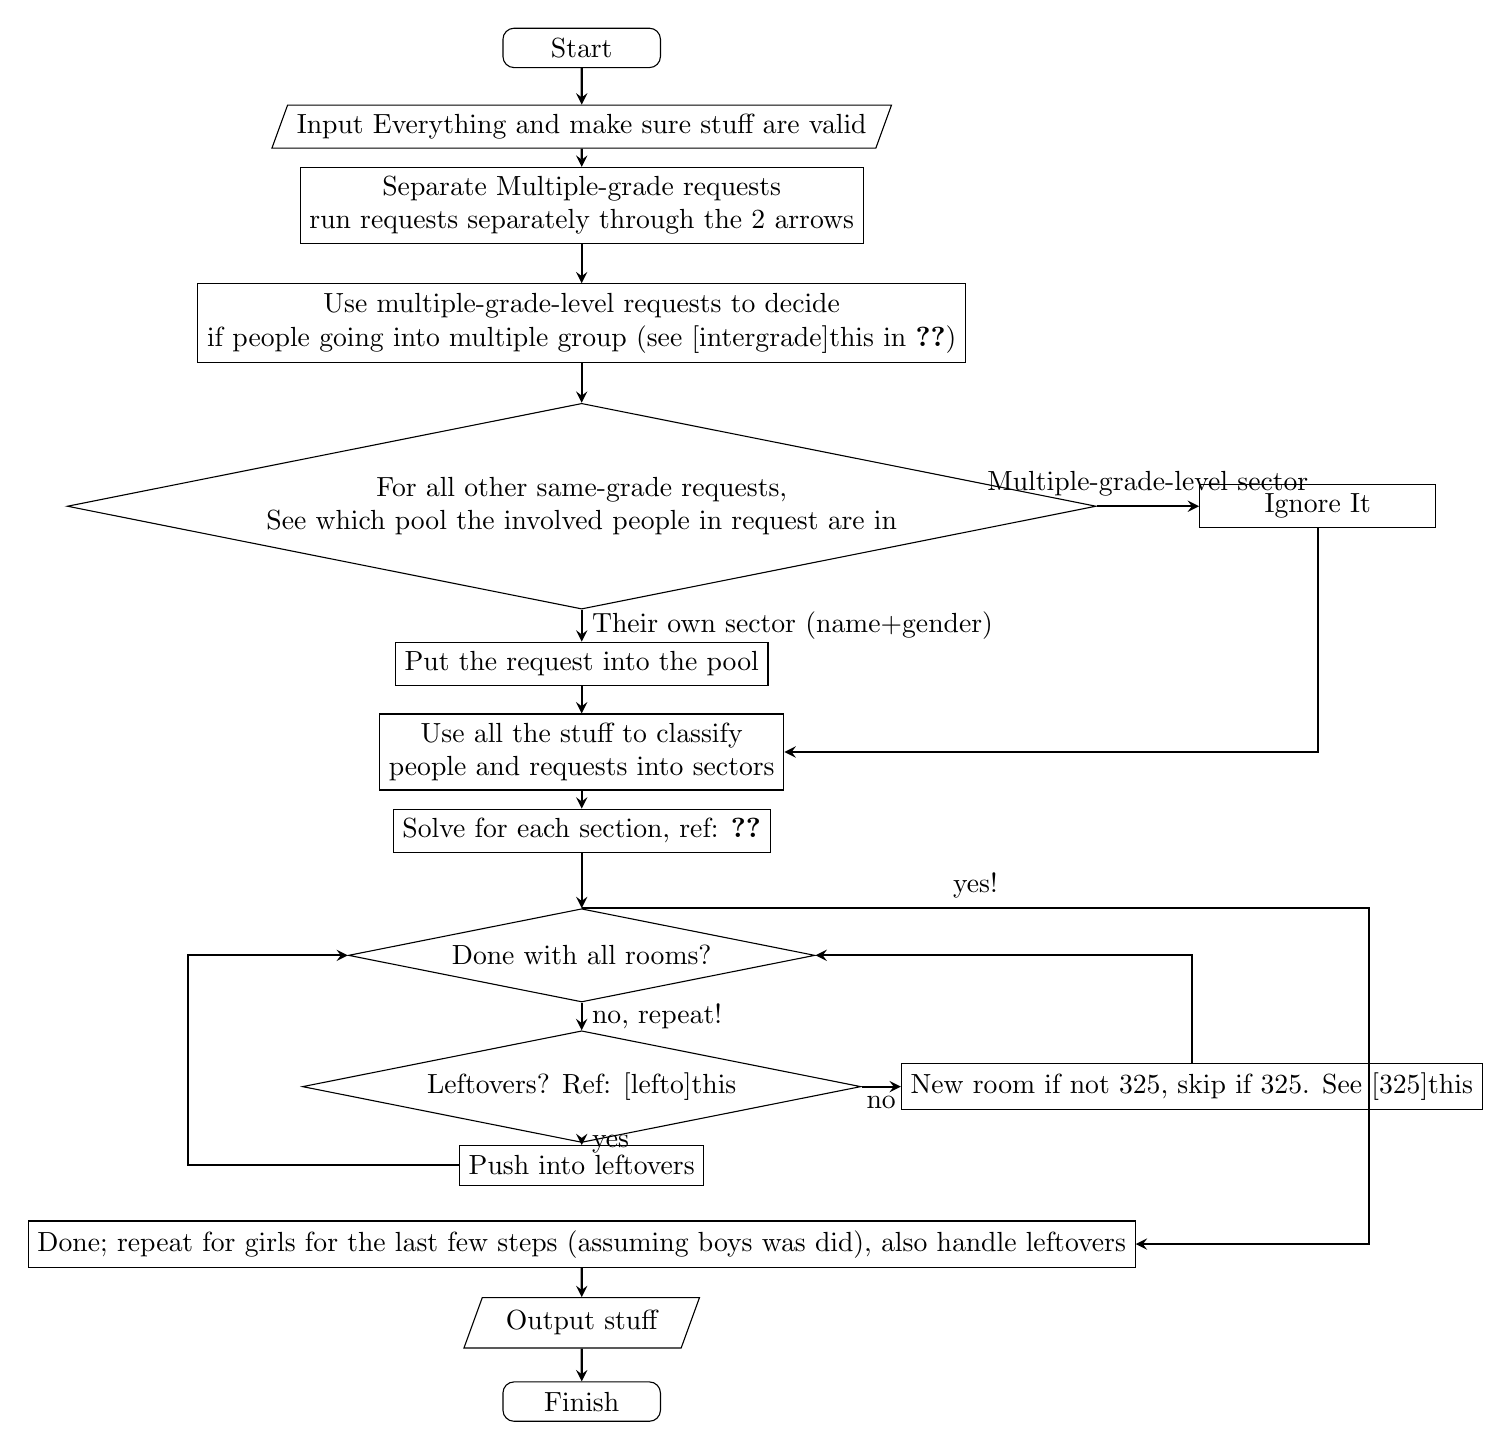
\begin{tikzpicture}[node distance=1cm]
			\node (start) [startstop] {Start};
			\node (in1) [io, below of=start] {Input Everything and make sure stuff are valid};
			\draw [arrow] (start) -- (in1);
			\node (multiple) [process, below of=in1]{\shortstack{Separate Multiple-grade requests\\run requests separately through the 2 arrows}};
			\draw [arrow] (in1) -- (multiple);
			\node (sepmultiple) [process, below=0.5cm of multiple] {\shortstack{Use multiple-grade-level requests to decide\\if people going into multiple group (see \hyperref[intergrade]{this} in \ref{sect})}};
			\node (samegrade) [decision, below=0.5cm of sepmultiple, aspect=5] {\shortstack{For all other same-grade requests,\\See which pool the involved people in request are in}};
			\draw [arrow] (multiple) -- (sepmultiple);
			\draw [arrow] (sepmultiple) -- (samegrade);
			\node (samegrade-req) [process, below of=samegrade, yshift=-1cm] {Put the request into the pool};
			\draw [arrow] (samegrade) -- node[anchor=west] {Their own sector (name+gender)} (samegrade-req);
			\node (samegrade-itreq) [process, right=1.3cm of samegrade] {Ignore It};
			\draw [arrow] (samegrade) -- node[anchor=south] {Multiple-grade-level sector} (samegrade-itreq);
			\node (class) [process, below=1em of samegrade-req] {\shortstack{Use all the stuff to classify\\people and requests into sectors}};
			\draw [arrow] (samegrade-req) -- (class);
			\draw [arrow] (samegrade-itreq) |- (class);
			\node (solve) [process, below of = class] {Solve for each section, ref: \ref{Algorithm}};
			\draw [arrow] (class) -- (solve);
			\node (done) [decision, below=2em of solve, aspect=5] {Done with all rooms?};
			\draw [arrow] (solve) -- (done);
			\node (leftovers) [decision, below=1em of done, aspect=5] {Leftovers? Ref: \hyperref[lefto]{this}};
			\node (pushleft) [process, below of=leftovers] {Push into leftovers};
			\draw [arrow] (done) -- node[anchor=west]{no, repeat!} (leftovers);
			\draw [arrow] (leftovers) -- node[anchor=west]{yes} (pushleft);
			\node (pushroom) [process, right=0.5cm of leftovers] {New room if not 325, skip if 325. See \hyperref[325]{this}};
			\draw [arrow] (leftovers) -- node[anchor=north]{no} (pushroom);
			\draw [arrow] (pushroom) |- (done);
			\draw [arrow] (pushleft) -- ++(-5,0) % From A go left
			|- (done.west); % Reach the left side of B
			\node (done1) [process, below of=pushleft] {Done; repeat for girls for the last few steps (assuming boys was did), also handle leftovers};
			\draw [arrow] (done.north) -- node[anchor=south]{yes!} ++(+10,0)
			|- (done1.east); % Reach the left side of B
			\node (output) [io, below of=done1] {Output stuff};
			\node (stop) [startstop, below of = output] {Finish};
			\draw [arrow] (done1) -- (output);
			\draw [arrow] (output) -- (stop);
	\end{tikzpicture}
	
	See the source code for more details.\index{Source code}
	\section{Concepts \& Featues}
	\subsection{Definitions}
	A \textbf{request} is a statement in the form ``$a$ wants to sleep with $b$''. The direction does not matter. If they
	requests each other (internally known as ``couples''), it is only counted as $1$ request. A request may carry a
	\textbf{priority} if it is across grade levels. \index{request} \index{priority}
	
	An \textbf{anti-request} is similar that says ``$a$ does not \emph{want to} sleep with $b$'' without a priority. See
	\hyperref[anti]{anti-requests in Sheets to Fill In} and \ref{Algorithm} for more info. \index{anti-request}
	
	A person, participant etc.\ is someone who is involved in the rooming.
	\index{participant}
	\subsection{Participant Identification}\index{participant}\index{identification}
	A participant is identified by its first name, last name, and his/hers grade level. There's duplicate names.
	\subsection{Sectoring}\index{sectors}\label{sect}
	\textbf{Definition.} Separate participants into groups:
	\begin{center}
		\begin{tabular}{c|c c c c}
			&$6$&$7$&$8$&multiple\\ \hline
			Boy&&&&\\
			Girl&&&&
		\end{tabular}
	\end{center}
	where every blank space inside represents a ``sector'' or group. 
	
	\subsubsection{``Multiple''  (aka. ``Inter-grade'') Sectors}\label{intergrade}\index{multiple-grade-level}
	
	Those are across grade levels. Requests (``pairs'') with high priorities are thrown in first, and then the low ones.
	If it gets stuck where the quota still allows $1$ empty spot but a pair of $2$ where neither person is already in the pool,
	it is skipped; however, if there is another pair with lower priority that has $1$ already in the pool, it is thrown in.
	
	\subsubsection{Leftovers} \index{leftovers ``other''} \label{lefto}
	
	Let's say you have $11$ people one sector. The algorithm extracts the first $8$ into $2$ rooms, but there are still $3$.
	They get thrown into a pool according to their gender named ``leftovers''. In the leftovers sector, people are not
	arranged but just put into there in the order their sectors go. Boys can never sleep with girls so there are separate
	leftover groups (kind of a mistake that it's implemented, there are only a few girls and they fit perfectly in one room
	last time).\index{Boys Can Never Sleep With Girls}
	
	\subsubsection{Ignored Requests}
	Boys cannot sleep with girls so requests across multiple genders are ignored.\index{Boys Can Never Sleep With Girls}
	
	Requests where one or more of the two people that are not in the multiple-grade-level pool are ignored.
	Same-grade-level requests are also thrown away in the multiple-grade-level pools.\index{same-grade-level requests}
	
	Anti-requests are ignored if the people involved are not in the same sector.
	
	\subsection{Special Rooms}\index{$325$}\label{325}
	Room numbers are reserved if such room number satisfying rules $325$, $*325$, or $3251$ are in the list, where $*$ is any digit ($0\sim9$), (only $3251$ not $325*$ to avoid skipping too much rooms).
	
	To disable $325$ checking, make the \verb|is325| function in main script always return \verb|false|. The reason for doing this by default cannot be disclosed.
	
	Chaperone rooms are marked at the end of each gender arrangement floor, by the numbers specified in the Student
	Info data entry sheet. Other extra rooms that has room numbers are marked as \verb|OTHER|. Do not confuse with \verb|other Boy/Girl| which 
	is the external term for leftovers.\index{chaperone rooms}\index{special rooms}\index{leftovers ``other''}
	
	\section{Output Format}
	\subsection{Arrangement Sheets}\index{arrangement sheets}
	\textbf{Example.} \texttt{1324|other Girl|2|b a 8|d c 8|x f 8|w2 z 8}
	
	Column \verb|A|: Room numbers.
	
	Column \verb|B|: Sector.
	
	Column \verb|C|: Room Ordinal in Sector -- starting from room 1 in each sector. \index{room ordinal in sector}
	
	Columns \verb|D, E, F, G (and more if you have more pople in a room)|: Names in Room.
	
	\subsection{Adjusting Rooms}\index{adjustments}
	
	To adjust people in rooms, use the generated arrangement sheets \index{arrangement sheets} -- fill in the small ``form'' to the right. The highlighted
	parts should be the cell \emph{address}, like \verb|A3|. They will swap if there is already a person in the ``to'' field and it
	will update all output sheets, although it is still dependent on the input sheets so do not delete them.
	
	To rename rooms, use the form below the previous form. Make sure there are no name collisions, although it is not that
	important. If you swap the names of two rooms, do
	\begin{center}
		\texttt{Rename A to C} (C may be a random name like \texttt{Temp 1})
		
		\texttt{Rename B to A}
		
		\texttt{Rename C (``Original'' A) to B}
	\end{center}
	
	To swap the rooms' locations on the sheet, simply do it. There are no line number references.
	
	To change room numbers, there are no simple ways to do it. Start over. \textbf{That is why you should log all your actions. The algorithm is deterministic even though room numbers change.}
	
	\section{Final Remarks}
	
	To just do the part for the greedy algorithm (for seating charts etc), use the following form:
	\begin{center}
		\includegraphics[width=0.8\linewidth]{"pic"}
	\end{center}
	and run the main script from that sheet (in this case only about $200$ lines are ran).
	
	Non-features: Larger size may fail in this program. Larger arrangements, such as buses \index{bus} are a non-feature.
	
	\chapter{Converting to a Word Document}\index{Word document}
	
	
	The first line of the sheet that you run the VBA script from is a header that you can put anything in that gets skipped during processing. Starting from the second line paste in stuff from Arrangement
	sheets as output of first program, skipping the first line, remove everything you don't want in a final sheet of Word table to send out. If you want to color-code room grids, the color should be in the first column.
	
	You may want to change up the sector names etc. Experiment with things to get the result you want.
	
	There will be three dialogue boxes that pop up, the first two of which are self-explanatory and the last of which basically means the number of rows in the table.
	\printindex
\end{document}